% Generated on 2025-04-15 17:44:06 by gEcon ver. 1.2.1 (2023-01-18)
% http://gecon.r-forge.r-project.org/

% Model name: baseline_NK

\section{Steady-state values}


\begin{tabular}{c|c|}
  & Steady-state value\\
\hline
$\epsilon^{\mathrm{G}}$ & 1 \\
$g^{\mathrm{1}}$ & 7.3514 \\
$g^{\mathrm{2}}$ & 4.9009 \\
$\lambda$ & 1.5467 \\
${m\!c}$ & 0.6667 \\
$\nu^{\mathrm{p}}$ & 1 \\
$\pi$ & 1 \\
$\pi^{\star}$ & 1 \\
$\pi^{\mathrm{obj}}$ & 1 \\
$q$ & 1.5467 \\
$r$ & 0.0351 \\
$B$ & 0 \\
$C$ & 0.3255 \\
${D\!i\!v}$ & 0.1601 \\
$G$ & 0.0865 \\
$I$ & 0.0684 \\
$K^{\mathrm{s}}$ & 2.7374 \\
$L^{\mathrm{s}}$ & 0.2279 \\
$Q$ & 1 \\
$R$ & 1.0101 \\
$T$ & 0.0865 \\
$U$ & -167.8256 \\
$W$ & 0.9837 \\
$Y$ & 0.4804 \\
$Y^{\mathrm{j}}$ & 0.4804 \\
$Y^{\mathrm{s}}$ & 0.4804 \\
$Z$ & 1 \\
\hline
\end{tabular}


\section{The solution of the 1st order perturbation}

\subsection*{Matrix $P$}

$$\bordermatrix{
~ & \epsilon^{\mathrm{G}}_{t-1} & \nu^{\mathrm{p}}_{t-1} & \pi_{t-1} & \pi^{\mathrm{obj}}_{t-1} & B_{t-1} & K^{\mathrm{s}}_{t-1} & R_{t-1} & Z_{t-1} \cr
\epsilon^{\mathrm{G}}_{t} & 0.949 & 0 & 0 & 0 & 0 & 0 & 0 & 0 \cr
\nu^{\mathrm{p}}_{t} & 0 & 0.908 & 0 & 0 & 0 & 0 & 0 & 0 \cr
\pi_{t} & -0.0001 & 0.0549 & 0.3347 & 0.3431 & 0 & -0.0399 & -1.1151 & -0.0644 \cr
\pi^{\mathrm{obj}}_{t} & 0 & 0 & 0 & 0.924 & 0 & 0 & 0 & 0 \cr
B_{t} & 0 & 0 & 0 & 0 & 0 & 0 & 0 & 0 \cr
K^{\mathrm{s}}_{t} & 0.0052 & 0.5527 & -1.2493 & 3.5068 & 0 & 0.4384 & -15.1013 & -0.4031 \cr
R_{t} & 0.0006 & 0.0147 & 0.0313 & 0.0717 & 0 & -0.0135 & 0.5465 & -0.011 \cr
Z_{t} & 0 & 0 & 0 & 0 & 0 & 0 & 0 & 0.823 \cr
}$$

\subsection*{Matrix $Q$}

$$\bordermatrix{
~ & \epsilon^{\mathrm{Z}} & \eta^{\mathrm{p}} & \eta^{\mathrm{R}} & \eta^{\pi} & \eta^{\mathrm{G}} \cr
\epsilon^{\mathrm{G}} & 0 & 0 & 0 & 0 & 1 \cr
\nu^{\mathrm{p}} & 0 & 0 & 0 & 0 & 0 \cr
\pi & -0.0783 & 0.0121 & -1.1604 & 0.3714 & -0.0001 \cr
\pi^{\mathrm{obj}} & 0 & 0 & 0 & 1 & 0 \cr
B & 0 & 0 & 0 & 0 & 0 \cr
K^{\mathrm{s}} & -0.4898 & -0.0064 & -15.7141 & 3.7952 & 0.0055 \cr
R & -0.0133 & -0.0002 & 0.5687 & 0.0776 & 0.0007 \cr
Z & 1 & 0 & 0 & 0 & 0 \cr
}$$

\subsection*{Matrix $R$}

$$\bordermatrix{
~ & \epsilon^{\mathrm{G}}_{t-1} & \nu^{\mathrm{p}}_{t-1} & \pi_{t-1} & \pi^{\mathrm{obj}}_{t-1} & B_{t-1} & K^{\mathrm{s}}_{t-1} & R_{t-1} & Z_{t-1} \cr
g^{\mathrm{1}}_{t} & 0.1474 & 0.9164 & -1.9772 & 5.4585 & 0 & -0.8826 & -15.6826 & -0.8627 \cr
g^{\mathrm{2}}_{t} & 0.1474 & 0.9164 & -1.9772 & 5.4585 & 0 & -0.8826 & -15.6826 & -0.8627 \cr
\lambda_{t} & 0.1179 & 0.1359 & 0.8044 & -2.1906 & 0 & -0.2745 & 9.2056 & -0.0385 \cr
{m\!c}_{t} & 0.0862 & 4.9707 & -10.2156 & 28.5786 & 0 & -4.181 & -122.7414 & -4.7402 \cr
\pi^{\star}_{t} & -0.0012 & 0.5419 & -1.3251 & 3.3865 & 0 & -0.3941 & -11.0059 & -0.636 \cr
q_{t} & 0.1179 & 0.1359 & 0.8044 & -2.1906 & 0 & -0.2745 & 9.2056 & -0.0385 \cr
r_{t} & 0.2504 & 9.6818 & -19.1237 & 53.542 & 0 & -8.6795 & -230.1009 & -7.5809 \cr
C_{t} & -0.0534 & 0.9651 & -2.6415 & 7.3533 & 0 & -0.6513 & -31.4584 & -0.8022 \cr
{D\!i\!v}_{t} & -0.0082 & -7.9544 & 11.5232 & -32.1937 & 0 & 4.8635 & 138.1234 & 6.6399 \cr
G_{t} & 0.949 & 0 & 0 & 0 & 0 & 0 & 0 & 0 \cr
I_{t} & 0.2078 & 22.1074 & -49.9721 & 140.272 & 0 & -21.4622 & -604.0515 & -16.1258 \cr
L^{\mathrm{s}}_{t} & 0.2346 & 6.7301 & -12.7258 & 35.662 & 0 & -5.4264 & -153.3707 & -5.2337 \cr
Q_{t} & 0 & 0 & 0 & 0 & 0 & 0 & 0 & 0 \cr
T_{t} & 0.949 & 0 & 0 & 0 & 11.5637 & 0 & 0 & 0 \cr
U_{t} & -0.0107 & -0.0272 & -0.0234 & 0.0592 & 0 & 0.0226 & -0.1954 & 0.0162 \cr
W_{t} & 0.0158 & 2.9517 & -6.3979 & 17.88 & 0 & -2.2531 & -76.7302 & -2.3471 \cr
Y_{t} & 0.1642 & 3.803 & -8.9081 & 24.9634 & 0 & -3.4985 & -107.3595 & -2.8406 \cr
Y^{\mathrm{j}}_{t} & 0.1642 & 4.711 & -8.9081 & 24.9634 & 0 & -3.4985 & -107.3595 & -2.8406 \cr
Y^{\mathrm{s}}_{t} & 0.1642 & 4.711 & -8.9081 & 24.9634 & 0 & -3.4985 & -107.3595 & -2.8406 \cr
}$$

\subsection*{Matrix $S$}

$$\bordermatrix{
~ & \epsilon^{\mathrm{Z}} & \eta^{\mathrm{p}} & \eta^{\mathrm{R}} & \eta^{\pi} & \eta^{\mathrm{G}} \cr
g^{\mathrm{1}} & -1.0482 & 0.1094 & -16.319 & 5.9075 & 0.1553 \cr
g^{\mathrm{2}} & -1.0482 & -0.0266 & -16.319 & 5.9075 & 0.1553 \cr
\lambda & -0.0468 & 0.0052 & 9.5791 & -2.3707 & 0.1243 \cr
{m\!c} & -5.7597 & -0.0537 & -127.7226 & 30.9292 & 0.0908 \cr
\pi^{\star} & -0.7728 & 0.1192 & -11.4526 & 3.6651 & -0.0012 \cr
q & -0.0468 & 0.0052 & 9.5791 & -2.3707 & 0.1243 \cr
r & -9.2112 & -0.0999 & -239.439 & 57.9459 & 0.2638 \cr
C & -0.9748 & -0.0144 & -32.735 & 7.9581 & -0.0563 \cr
{D\!i\!v} & 8.0679 & 0.0612 & 143.7288 & -34.8417 & -0.0086 \cr
G & 0 & 0 & 0 & 0 & 1 \cr
I & -19.5939 & -0.2554 & -628.5656 & 151.8096 & 0.2189 \cr
L^{\mathrm{s}} & -6.3593 & -0.066 & -159.5949 & 38.5953 & 0.2472 \cr
Q & 0 & 0 & 0 & 0 & 0 \cr
T & 0 & 0 & 0 & 0 & 1 \cr
U & 0.0197 & -0.0003 & -0.2033 & 0.0641 & -0.0113 \cr
W & -2.8519 & -0.0339 & -79.8442 & 19.3506 & 0.0167 \cr
Y & -3.4515 & -0.0462 & -111.7164 & 27.0167 & 0.173 \cr
Y^{\mathrm{j}} & -3.4515 & -0.0462 & -111.7164 & 27.0167 & 0.173 \cr
Y^{\mathrm{s}} & -3.4515 & -0.0462 & -111.7164 & 27.0167 & 0.173 \cr
}$$


\section{Model statistics}

\subsection{Basic statistics}

\begin{tabular}{c|c|c|c|c|}
  & Steady-state value & Std. dev. & Variance & Loglin\\
\hline
$\epsilon^{\mathrm{G}}$ & 1 & 1.3033 & 1.6986 & Y    \\
$g^{\mathrm{1}}$ & 7.3514 & 20.4264 & 417.2364 & Y    \\
$g^{\mathrm{2}}$ & 4.9009 & 20.4261 & 417.2261 & Y    \\
$\lambda$ & 1.5467 & 12.2819 & 150.8456 & Y    \\
${m\!c}$ & 0.6667 & 127.9129 & 16361.6994 & Y    \\
$\nu^{\mathrm{p}}$ & 1 & 0 & 0 & Y    \\
$\pi$ & 1 & 1.2289 & 1.5103 & Y    \\
$\pi^{\star}$ & 1 & 11.8863 & 141.285 & Y    \\
$\pi^{\mathrm{obj}}$ & 1 & 1.2958 & 1.6792 & Y    \\
$q$ & 1.5467 & 12.2819 & 150.8456 & Y    \\
$r$ & 0.0351 & 246.1531 & 60591.3569 & Y    \\
$B$ & 0 & 0 & 0 & N    \\
$C$ & 0.3255 & 30.8464 & 951.4999 & Y    \\
${D\!i\!v}$ & 0.1601 & 145.1625 & 21072.1497 & Y    \\
$G$ & 0.0865 & 1.3033 & 1.6986 & Y    \\
$I$ & 0.0684 & 635.6189 & 404011.446 & Y    \\
$K^{\mathrm{s}}$ & 2.7374 & 20.0049 & 400.1958 & Y    \\
$L^{\mathrm{s}}$ & 0.2279 & 161.2555 & 26003.3342 & Y    \\
$Q$ & 1 & 0 & 0 & Y    \\
$R$ & 1.0101 & 0.6891 & 0.4749 & Y    \\
$T$ & 0.0865 & 1.3033 & 1.6986 & Y    \\
$U$ & -167.8256 & 0.5474 & 0.2997 & Y    \\
$W$ & 0.9837 & 77.7077 & 6038.4897 & Y    \\
$Y$ & 0.4804 & 110.761 & 12268.0006 & Y    \\
$Y^{\mathrm{j}}$ & 0.4804 & 110.761 & 12268.0006 & Y    \\
$Y^{\mathrm{s}}$ & 0.4804 & 110.761 & 12268.0006 & Y    \\
$Z$ & 1 & 1.227 & 1.5056 & Y    \\
\hline
\end{tabular}


\subsection{Correlation matrix}

\begin{tabular}{c|cccccccccccccccccccccccc|}
  & $\epsilon^{\mathrm{G}}$ & $g^{\mathrm{1}}$ & $g^{\mathrm{2}}$ & $\lambda$ & ${m\!c}$ & $\pi$ & $\pi^{\star}$ & $\pi^{\mathrm{obj}}$ & $q$ & $r$ & $C$ & ${D\!i\!v}$ & $G$ & $I$ & $K^{\mathrm{s}}$ & $L^{\mathrm{s}}$ & $R$ & $T$ & $U$ & $W$ & $Y$ & $Y^{\mathrm{j}}$ & $Y^{\mathrm{s}}$ & $Z$\\
\hline
$\epsilon^{\mathrm{G}}$ & 1 & 0.009 & 0.009 & 0.013 & 0 & -0.001 & -0.001 & 0 & 0.013 & 0.001 & -0.003 & 0.001 & 1 & 0 & 0 & 0.001 & 0.001 & 1 & -0.027 & 0 & 0.001 & 0.001 & 0.001 & 0 \\
$g^{\mathrm{1}}$ &  & 1 & 1 & -0.134 & 0.94 & 0.771 & 0.958 & 0.148 & -0.134 & 0.959 & 0.828 & -0.947 & 0.009 & 0.948 & 0.141 & 0.947 & -0.121 & 0.009 & -0.312 & 0.909 & 0.931 & 0.931 & 0.931 & -0.031 \\
$g^{\mathrm{2}}$ &  &  & 1 & -0.134 & 0.94 & 0.771 & 0.958 & 0.148 & -0.134 & 0.959 & 0.828 & -0.947 & 0.009 & 0.948 & 0.141 & 0.947 & -0.121 & 0.009 & -0.312 & 0.909 & 0.931 & 0.931 & 0.931 & -0.031 \\
$\lambda$ &  &  &  & 1 & -0.445 & -0.626 & -0.411 & -0.243 & 1 & -0.387 & -0.659 & 0.426 & 0.013 & -0.422 & -0.999 & -0.424 & 0.917 & 0.013 & -0.896 & -0.521 & -0.469 & -0.469 & -0.469 & -0.005 \\
${m\!c}$ &  &  &  &  & 1 & 0.899 & 0.994 & 0.109 & -0.445 & 0.998 & 0.967 & -1 & 0 & 1 & 0.452 & 1 & -0.449 & 0 & 0.001 & 0.996 & 0.999 & 0.999 & 0.999 & -0.028 \\
$\pi$ &  &  &  &  &  & 1 & 0.888 & 0.283 & -0.626 & 0.881 & 0.933 & -0.894 & -0.001 & 0.891 & 0.633 & 0.893 & -0.559 & -0.001 & 0.253 & 0.917 & 0.905 & 0.905 & 0.905 & -0.071 \\
$\pi^{\star}$ &  &  &  &  &  &  & 1 & 0.189 & -0.411 & 0.994 & 0.952 & -0.995 & -0.001 & 0.994 & 0.418 & 0.995 & -0.381 & -0.001 & -0.032 & 0.987 & 0.993 & 0.993 & 0.993 & -0.051 \\
$\pi^{\mathrm{obj}}$ &  &  &  &  &  &  &  & 1 & -0.243 & 0.095 & 0.161 & -0.105 & 0 & 0.103 & 0.238 & 0.104 & 0.16 & 0 & 0.243 & 0.128 & 0.115 & 0.115 & 0.115 & 0 \\
$q$ &  &  &  &  &  &  &  &  & 1 & -0.387 & -0.659 & 0.426 & 0.013 & -0.422 & -0.999 & -0.424 & 0.917 & 0.013 & -0.896 & -0.521 & -0.469 & -0.469 & -0.469 & -0.005 \\
$r$ &  &  &  &  &  &  &  &  &  & 1 & 0.949 & -0.999 & 0.001 & 0.999 & 0.394 & 0.999 & -0.397 & 0.001 & -0.062 & 0.989 & 0.996 & 0.996 & 0.996 & -0.018 \\
$C$ &  &  &  &  &  &  &  &  &  &  & 1 & -0.961 & -0.003 & 0.96 & 0.664 & 0.961 & -0.639 & -0.003 & 0.256 & 0.985 & 0.973 & 0.973 & 0.973 & -0.016 \\
${D\!i\!v}$ &  &  &  &  &  &  &  &  &  &  &  & 1 & 0.001 & -1 & -0.434 & -1 & 0.432 & 0.001 & 0.019 & -0.994 & -0.998 & -0.998 & -0.998 & 0.04 \\
$G$ &  &  &  &  &  &  &  &  &  &  &  &  & 1 & 0 & 0 & 0.001 & 0.001 & 1 & -0.027 & 0 & 0.001 & 0.001 & 0.001 & 0 \\
$I$ &  &  &  &  &  &  &  &  &  &  &  &  &  & 1 & 0.428 & 1 & -0.429 & 0 & -0.024 & 0.994 & 0.999 & 0.999 & 0.999 & -0.01 \\
$K^{\mathrm{s}}$ &  &  &  &  &  &  &  &  &  &  &  &  &  &  & 1 & 0.431 & -0.918 & 0 & 0.891 & 0.527 & 0.475 & 0.475 & 0.475 & -0.03 \\
$L^{\mathrm{s}}$ &  &  &  &  &  &  &  &  &  &  &  &  &  &  &  & 1 & -0.431 & 0.001 & -0.022 & 0.994 & 0.999 & 0.999 & 0.999 & -0.021 \\
$R$ &  &  &  &  &  &  &  &  &  &  &  &  &  &  &  &  & 1 & 0.001 & -0.79 & -0.517 & -0.471 & -0.471 & -0.471 & -0.024 \\
$T$ &  &  &  &  &  &  &  &  &  &  &  &  &  &  &  &  &  & 1 & -0.027 & 0 & 0.001 & 0.001 & 0.001 & 0 \\
$U$ &  &  &  &  &  &  &  &  &  &  &  &  &  &  &  &  &  &  & 1 & 0.088 & 0.029 & 0.029 & 0.029 & 0.031 \\
$W$ &  &  &  &  &  &  &  &  &  &  &  &  &  &  &  &  &  &  &  & 1 & 0.998 & 0.998 & 0.998 & -0.019 \\
$Y$ &  &  &  &  &  &  &  &  &  &  &  &  &  &  &  &  &  &  &  &  & 1 & 1 & 1 & -0.011 \\
$Y^{\mathrm{j}}$ &  &  &  &  &  &  &  &  &  &  &  &  &  &  &  &  &  &  &  &  &  & 1 & 1 & -0.011 \\
$Y^{\mathrm{s}}$ &  &  &  &  &  &  &  &  &  &  &  &  &  &  &  &  &  &  &  &  &  &  & 1 & -0.011 \\
$Z$ &  &  &  &  &  &  &  &  &  &  &  &  &  &  &  &  &  &  &  &  &  &  &  & 1 \\
\hline
\end{tabular}


\subsection{Cross correlations with the reference variable ($\pi$)}

\begin{tabular}{c|c|c|c|c|c|c|c|c|c|c|c|c|}
  & $\sigma[\cdot]$ rel. to $\sigma[\pi]$ & $\pi_{t-5}$ & $\pi_{t-4}$ & $\pi_{t-3}$ & $\pi_{t-2}$ & $\pi_{t-1}$ & $\pi_{t}$ & $\pi_{t+1}$ & $\pi_{t+2}$ & $\pi_{t+3}$ & $\pi_{t+4}$ & $\pi_{t+5}$\\
\hline
$\epsilon^{\mathrm{G}}_{t}$ & 1.061 & 0 & -0.001 & -0.001 & -0.001 & -0.002 & -0.001 & -0.001 & 0 & 0 & 0 & 0 \\
$g^{\mathrm{1}}_{t}$ & 16.621 & 0.015 & 0.037 & 0.075 & 0.152 & 0.329 & 0.771 & -0.358 & -0.245 & -0.186 & -0.146 & -0.116 \\
$g^{\mathrm{2}}_{t}$ & 16.621 & 0.015 & 0.037 & 0.075 & 0.152 & 0.328 & 0.771 & -0.358 & -0.245 & -0.186 & -0.146 & -0.116 \\
$\lambda_{t}$ & 9.994 & 0.276 & 0.32 & 0.342 & 0.301 & 0.081 & -0.626 & -0.476 & -0.367 & -0.278 & -0.204 & -0.142 \\
${m\!c}_{t}$ & 104.084 & -0.076 & -0.072 & -0.047 & 0.034 & 0.265 & 0.899 & -0.161 & -0.113 & -0.091 & -0.077 & -0.067 \\
$\pi_{t}$ & 1 & -0.116 & -0.113 & -0.083 & 0.011 & 0.277 & 1 & 0.277 & 0.011 & -0.083 & -0.113 & -0.116 \\
$\pi^{\star}_{t}$ & 9.672 & -0.066 & -0.059 & -0.031 & 0.051 & 0.277 & 0.888 & -0.196 & -0.121 & -0.09 & -0.075 & -0.065 \\
$\pi^{\mathrm{obj}}_{t}$ & 1.054 & -0.051 & -0.035 & -0.009 & 0.035 & 0.116 & 0.283 & 0.21 & 0.147 & 0.095 & 0.052 & 0.018 \\
$q_{t}$ & 9.994 & 0.276 & 0.32 & 0.342 & 0.301 & 0.081 & -0.626 & -0.476 & -0.367 & -0.278 & -0.204 & -0.142 \\
$r_{t}$ & 200.298 & -0.058 & -0.051 & -0.024 & 0.056 & 0.278 & 0.881 & -0.2 & -0.143 & -0.113 & -0.094 & -0.079 \\
$C_{t}$ & 25.1 & -0.142 & -0.151 & -0.137 & -0.057 & 0.199 & 0.933 & 0 & 0.009 & 0.003 & -0.007 & -0.016 \\
${D\!i\!v}_{t}$ & 118.121 & 0.07 & 0.065 & 0.04 & -0.041 & -0.27 & -0.894 & 0.173 & 0.122 & 0.098 & 0.083 & 0.071 \\
$G_{t}$ & 1.061 & 0 & -0.001 & -0.001 & -0.001 & -0.002 & -0.001 & -0.001 & 0 & 0 & 0 & 0 \\
$I_{t}$ & 517.212 & -0.068 & -0.064 & -0.038 & 0.043 & 0.27 & 0.891 & -0.177 & -0.126 & -0.1 & -0.084 & -0.072 \\
$K^{\mathrm{s}}_{t}$ & 16.278 & -0.275 & -0.319 & -0.341 & -0.299 & -0.077 & 0.633 & 0.476 & 0.365 & 0.276 & 0.202 & 0.14 \\
$L^{\mathrm{s}}_{t}$ & 131.216 & -0.069 & -0.064 & -0.039 & 0.042 & 0.27 & 0.893 & -0.175 & -0.124 & -0.099 & -0.084 & -0.072 \\
$R_{t}$ & 0.561 & 0.256 & 0.305 & 0.336 & 0.308 & 0.109 & -0.559 & -0.395 & -0.297 & -0.226 & -0.17 & -0.123 \\
$T_{t}$ & 1.061 & 0 & -0.001 & -0.001 & -0.001 & -0.002 & -0.001 & -0.001 & 0 & 0 & 0 & 0 \\
$U_{t}$ & 0.445 & -0.27 & -0.321 & -0.358 & -0.351 & -0.22 & 0.253 & 0.606 & 0.467 & 0.359 & 0.269 & 0.194 \\
$W_{t}$ & 63.232 & -0.099 & -0.1 & -0.078 & 0.003 & 0.244 & 0.917 & -0.107 & -0.072 & -0.06 & -0.054 & -0.05 \\
$Y_{t}$ & 90.128 & -0.083 & -0.081 & -0.057 & 0.024 & 0.258 & 0.905 & -0.145 & -0.101 & -0.081 & -0.07 & -0.062 \\
$Y^{\mathrm{j}}_{t}$ & 90.128 & -0.083 & -0.081 & -0.057 & 0.024 & 0.258 & 0.905 & -0.145 & -0.101 & -0.081 & -0.07 & -0.062 \\
$Y^{\mathrm{s}}_{t}$ & 90.128 & -0.083 & -0.081 & -0.057 & 0.024 & 0.258 & 0.905 & -0.145 & -0.101 & -0.081 & -0.07 & -0.062 \\
$Z_{t}$ & 0.998 & 0.009 & 0.003 & -0.006 & -0.02 & -0.04 & -0.071 & -0.047 & -0.027 & -0.013 & -0.002 & 0.006 \\
\hline
\end{tabular}


\subsection{Autocorrelations}

\begin{tabular}{c|ccccc|}
  & Lag 1 & Lag 2 & Lag 3 & Lag 4 & Lag 5\\
\hline
$\epsilon^{\mathrm{G}}$ & 0.713 & 0.471 & 0.271 & 0.109 & -0.017 \\
$g^{\mathrm{1}}$ & -0.071 & -0.04 & -0.035 & -0.037 & -0.04 \\
$g^{\mathrm{2}}$ & -0.071 & -0.04 & -0.035 & -0.037 & -0.04 \\
$\lambda$ & 0.681 & 0.438 & 0.246 & 0.095 & -0.022 \\
${m\!c}$ & -0.121 & -0.08 & -0.062 & -0.052 & -0.045 \\
$\pi$ & 0.277 & 0.011 & -0.083 & -0.113 & -0.116 \\
$\pi^{\star}$ & -0.142 & -0.08 & -0.056 & -0.045 & -0.039 \\
$\pi^{\mathrm{obj}}$ & 0.703 & 0.456 & 0.253 & 0.092 & -0.032 \\
$q$ & 0.681 & 0.438 & 0.246 & 0.095 & -0.022 \\
$r$ & -0.124 & -0.082 & -0.063 & -0.053 & -0.045 \\
$C$ & -0.034 & -0.024 & -0.028 & -0.036 & -0.042 \\
${D\!i\!v}$ & -0.122 & -0.081 & -0.063 & -0.052 & -0.045 \\
$G$ & 0.713 & 0.471 & 0.271 & 0.109 & -0.017 \\
$I$ & -0.122 & -0.081 & -0.063 & -0.053 & -0.045 \\
$K^{\mathrm{s}}$ & 0.677 & 0.433 & 0.242 & 0.093 & -0.023 \\
$L^{\mathrm{s}}$ & -0.123 & -0.081 & -0.063 & -0.052 & -0.045 \\
$R$ & 0.651 & 0.406 & 0.221 & 0.078 & -0.031 \\
$T$ & 0.713 & 0.471 & 0.271 & 0.109 & -0.017 \\
$U$ & 0.832 & 0.539 & 0.308 & 0.125 & -0.016 \\
$W$ & -0.105 & -0.07 & -0.056 & -0.049 & -0.045 \\
$Y$ & -0.117 & -0.078 & -0.061 & -0.052 & -0.045 \\
$Y^{\mathrm{j}}$ & -0.117 & -0.078 & -0.061 & -0.052 & -0.045 \\
$Y^{\mathrm{s}}$ & -0.117 & -0.078 & -0.061 & -0.052 & -0.045 \\
$Z$ & 0.644 & 0.368 & 0.159 & 0.006 & -0.102 \\
\hline
\end{tabular}



\pagebreak

\section{Impulse response functions}

\begin{figure}[h]
\begin{minipage}{0.5\textwidth}
\vspace*{-3em}
\centering
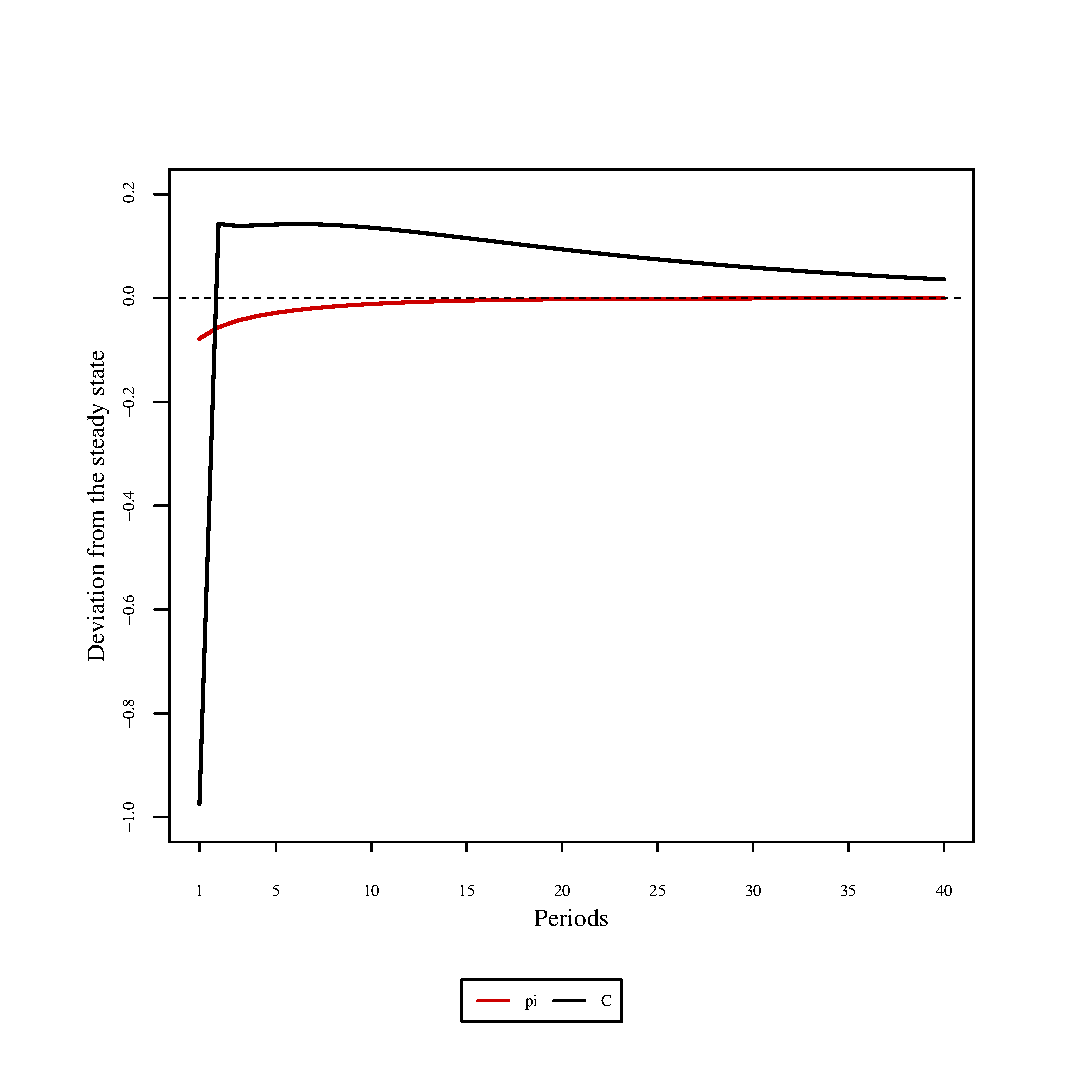
\includegraphics[width=0.99\textwidth, scale=0.55]{plots/plot_76.eps}
\caption{Impulse responses ($\pi, C$) to $\epsilon^{\mathrm{Z}}$ shock}
\end{minipage}
\begin{minipage}{0.5\textwidth}
\vspace*{-3em}
\centering
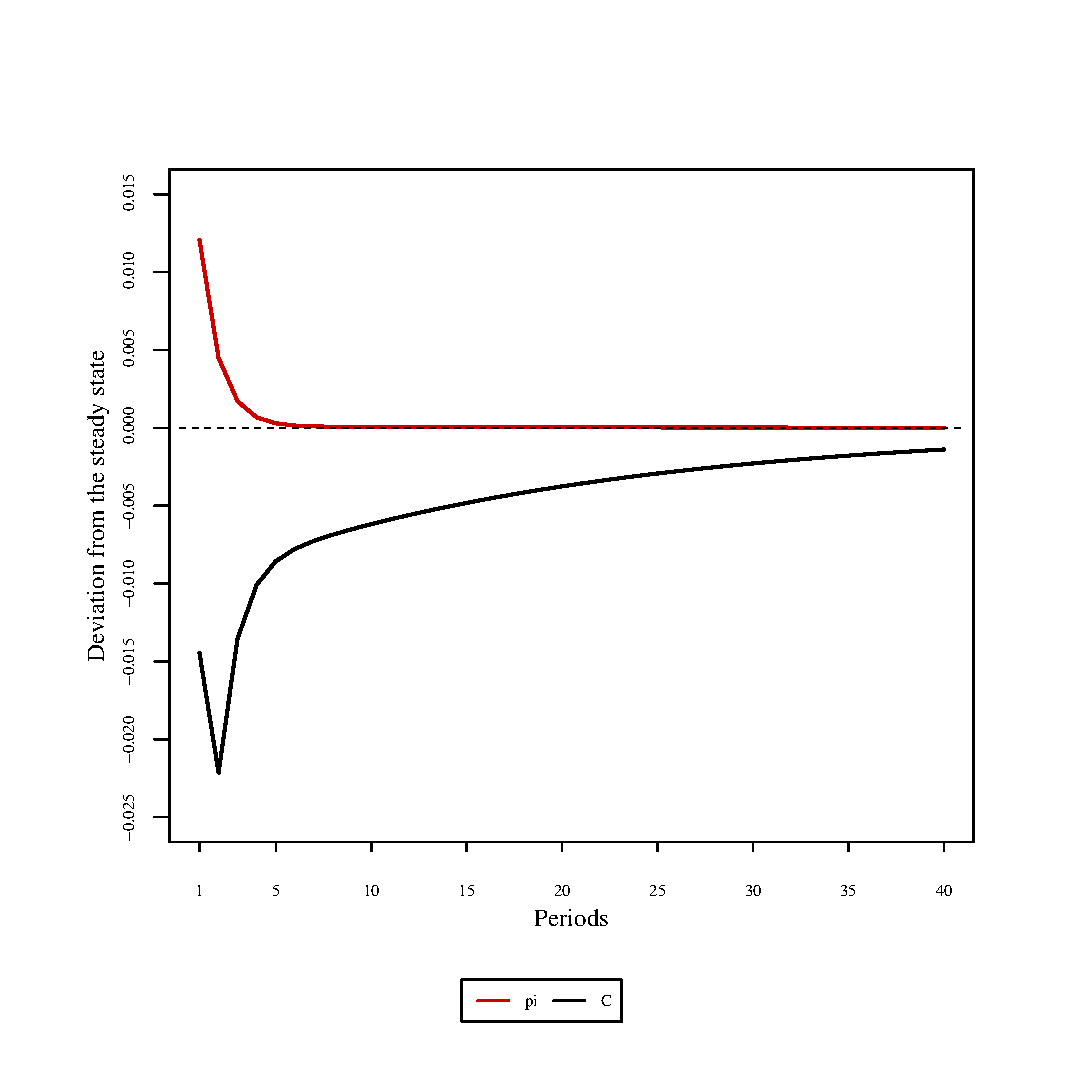
\includegraphics[width=0.99\textwidth, scale=0.55]{plots/plot_77.eps}
\caption{Impulse responses ($\pi, C$) to $\eta^{\mathrm{p}}$ shock}
\end{minipage}
\end{figure}

\begin{figure}[h]
\begin{minipage}{0.5\textwidth}
\vspace*{-3em}
\centering
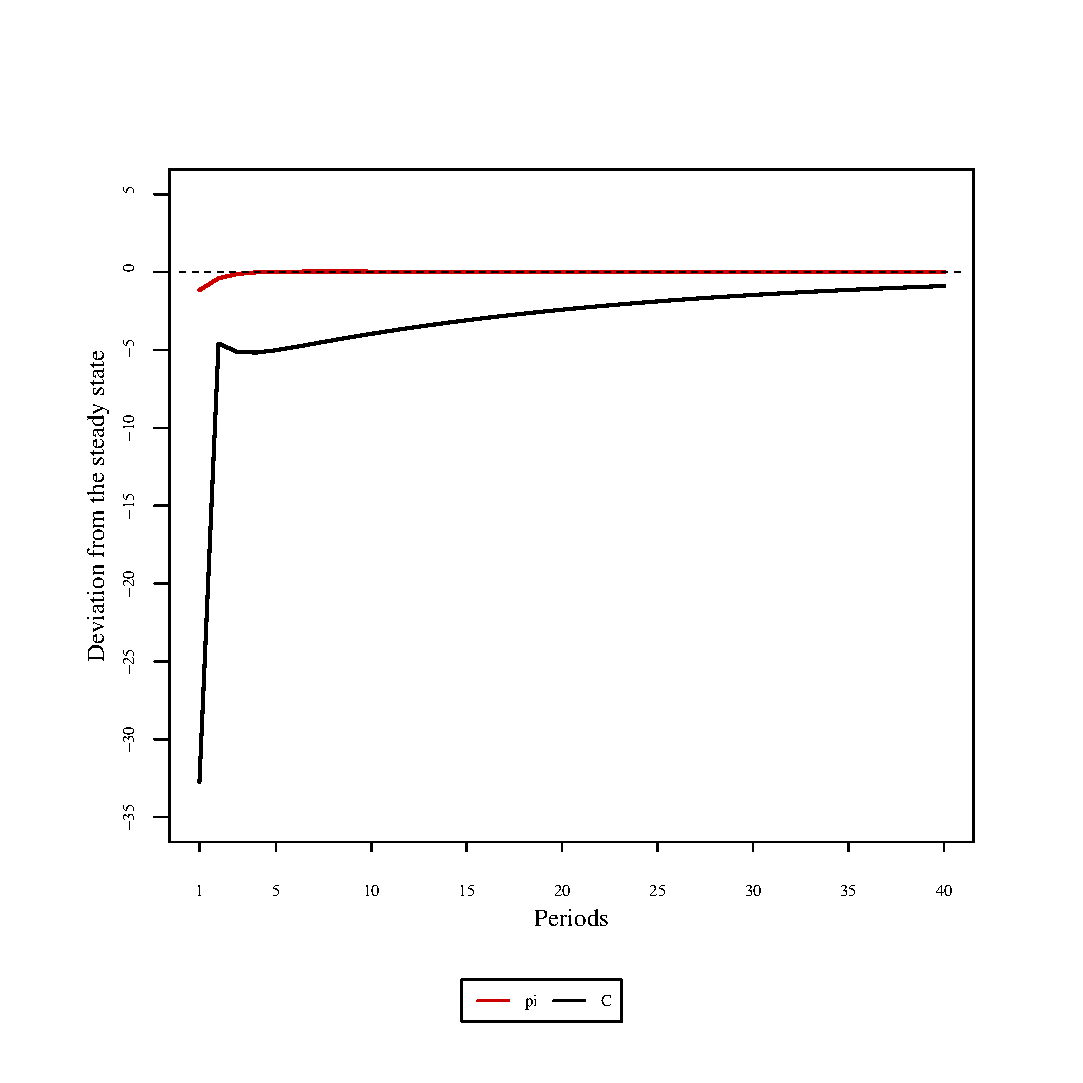
\includegraphics[width=0.99\textwidth, scale=0.55]{plots/plot_78.eps}
\caption{Impulse responses ($\pi, C$) to $\eta^{\mathrm{R}}$ shock}
\end{minipage}
\begin{minipage}{0.5\textwidth}
\vspace*{-3em}
\centering
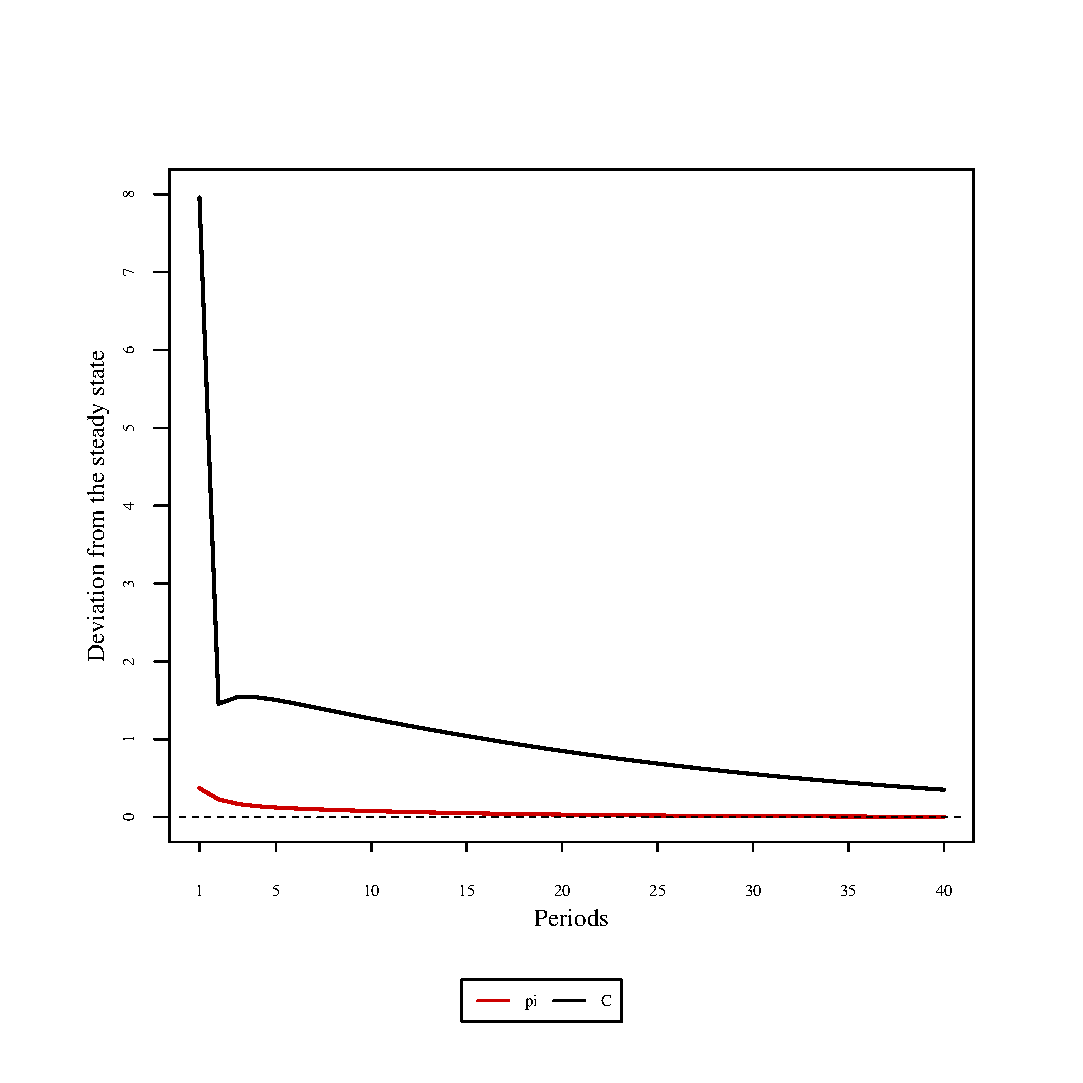
\includegraphics[width=0.99\textwidth, scale=0.55]{plots/plot_79.eps}
\caption{Impulse responses ($\pi, C$) to $\eta^{\pi}$ shock}
\end{minipage}
\end{figure}

\pagebreak

\begin{figure}[h]
\centering
\begin{minipage}{0.5\textwidth}
\vspace*{-3em}
\centering
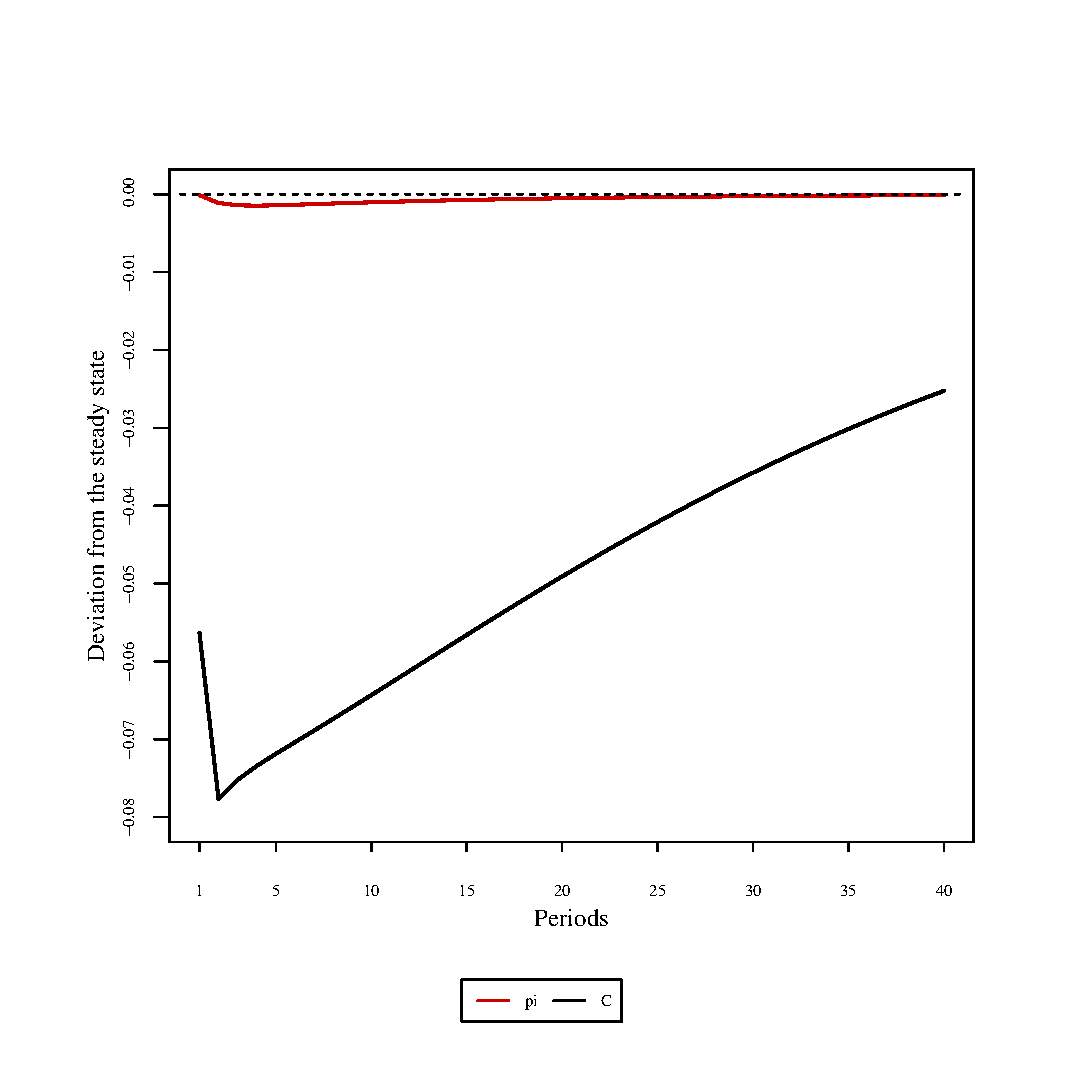
\includegraphics[width=0.99\textwidth, scale=0.55]{plots/plot_80.eps}
\caption{Impulse responses ($\pi, C$) to $\eta^{\mathrm{G}}$ shock}
\end{minipage}
\end{figure}
